\subsection{Cost functions}
\begin{frame}\frametitle{\subsecname}
\mode<article>{
A cost function $e\tyxw$, quantifies the discrepancy between the model's prediction $y(\vec x; \vec w)$ and the label $y_T$ which $\vec x$ is assigned to.
}
Choosing a cost function accounts for 
\begin{enumerate}
\item the type of problem (i.e. regression vs. classification), 
\item how the model is penalized for different types of mistakes it can make such as:
small errors are tolerable, large errors are penalized less, etc.
\end{enumerate}
\mode<article>{
The choice of cost function has a direct effect on how the model learns. For example, we will later see in gradient-based learning how the error function can modulate how fast or slow a model learns.
}
\end{frame}

\subsubsection{Cost functions for Regression}

\begin{frame}\frametitle{\subsecname}

  \begin{tabular}{c c c}
    \parbox{4cm}{
      \[ \underbrace{\vec{x}
          \in \mathbb{R}^N
      }_{\text{feature vector}}
      \longrightarrow 
      \underbrace{y
      \in \mathbb{R}
      }_{\substack{\text{scalar}\\ \text{attribute}}}
      \]}
    & & 
    \parbox{8cm}{\footnotesize
      \begin{tabular}{l l}
	$y_T(\vec x)$: & true value of attribute \\
	$y(\vec{x}; \vec w)$: & predicted value of attribute \\
					& (e.g. by MLP)
      \end{tabular}
    }
  \end{tabular}
     \pause

  \begin{block}{individual cost $e\tyxw$}
    \begin{center} 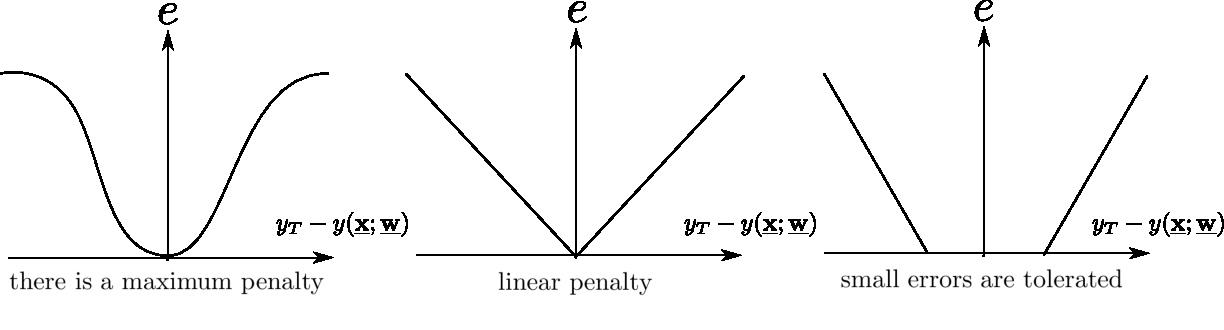
\includegraphics[width=12cm]{img/section1_fig17_v2.pdf} \end{center}
  \end{block}
\end{frame}

\begin{frame}\frametitle{Quadratic vs. linear error}

\begin{figure}[ht]
     \centering
     \savebox{\imagebox}{
	 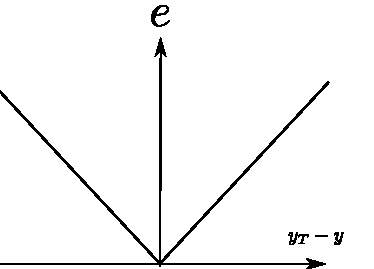
\includegraphics[width=0.4\textwidth]{img/section1_fig17_linear}}%
     \begin{subfigure}[t]{0.45\textwidth}
         \centering
         \usebox{\imagebox}% Place largest image
         \caption{linear error}
         \label{fig:quadratic}
     \end{subfigure}
     \hfill
     \begin{subfigure}[t]{0.45\textwidth}
         \centering
         \raisebox{\dimexpr.5\ht\imagebox-.5\height}{% Raise smaller image into place
         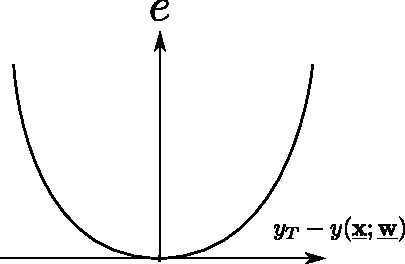
\includegraphics[width=0.99\textwidth]{img/section1_fig17_quadratic}
         }
         \caption{qudratic error}
         \label{fig:linear}
     \end{subfigure}
     \mode<article>{
     \caption{quadratic vs. linear error}
     }
	 \label{fig:quadratic_vs_linear}
\end{figure}


\begin{equation}
e_{\text{quadratic}}\tyxw := \frac{1}{2} \Big( y_{T}(\vec x) - y(\vec x;\vec w)\Big)^{2}
\label{eq:quadratic_error}
\end{equation}

\begin{equation}
e_{\text{linear}}\tyxw := \Big| y_{T}(\vec x) - y(\vec x;\vec w)\Big|
\label{eq:linear_error}
\end{equation}
\mode<article>{
The purpose of having $\frac{1}{2}$ in \eqref{eq:quadratic_error} is for convenience for when we calculate the derivative later. 
Both the quadratic and linear cost functions are symmetric. They therefore yield the same error regardless of the sign. However, the differences between them are:
}
\end{frame}
\begin{frame}\frametitle{Quadratic vs. linear error}

\mode<presentation>{
	\placeimage{8.5}{1.2}{img/section1_fig17_quadratic}{width=2.5cm}
	\placeimage{12.5}{.9}{img/section1_fig17_linear}{width=2.5cm}
}

\begin{table}[h]
\centering
\caption{Differences between quadratic and linear cost}
\begin{tabular}{|c|c|}
\hline
quadratic                                                                                                    & linear                                                                                                  \\ \hline \hline
\begin{tabular}[c]{@{}c@{}}larger error $\leadsto$ larger penalty\\  (sensitive to outliers)\end{tabular} & \begin{tabular}[c]{@{}c@{}}constant increase in error\\  (more stable, robust to outliers)\end{tabular} \\ \hline
\begin{tabular}[c]{@{}c@{}}converges faster\\ but slow convergence\\ for small errors\end{tabular}           & constant convergence rate                                                                               \\ \hline
differentiable everywhere                                                                                    & \begin{tabular}[c]{@{}c@{}}not differentiable at zero\\ (not a huge problem)\end{tabular}               \\ \hline
\begin{tabular}[c]{@{}c@{}}max. likelihood of\\ Gaussian variable\end{tabular}                               &                                                                                                         \\ \hline
\end{tabular}
\end{table}

\end{frame}

\newpage



\begin{frame}\frametitle{Relation between quadratic error and Gaussian labels}

\mode<article>{
\textbf{Relation between quadratic error and Gaussian labels}

}

Assume labels $y_T$ are conditionally Gaussian:

\begin{equation}
P(y_T|\vec x) = \mathcal{N}(y_T|\underbrace{y(\vec x;\vec w)}_{= \mu},\sigma^2)
\label{eq:gaussian_labels}
\end{equation}

\mode<article>{
Using the quadratic cost leads to a solution that corresponds to the same solution found from maximizing the (log-)likelihood\footnote{often, the log-likelihood is maximized for computational efficiency as the log replaces the product with a sum.} of the Gaussian labels:
}
\slidesonly{
\only<1>{
    \begin{center}
        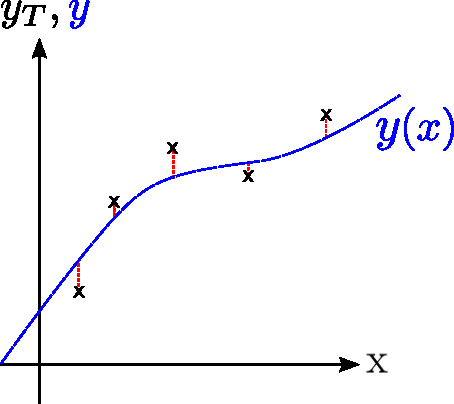
\includegraphics[height=4cm]{img/Regression_example}
    \end{center}
}
}
\only<2>{
    \begin{center}
        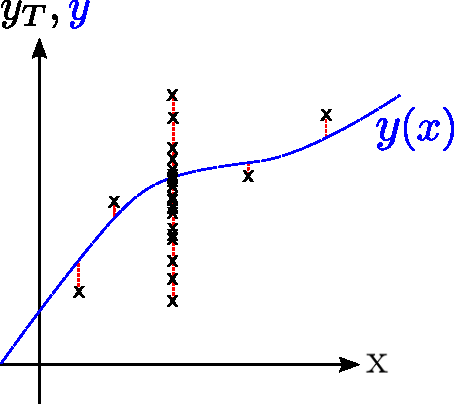
\includegraphics[height=4cm]{img/Regression_example_dense}
    \end{center}
}
\only<3>{
%\begin{figure}[h]
     %\centering
	%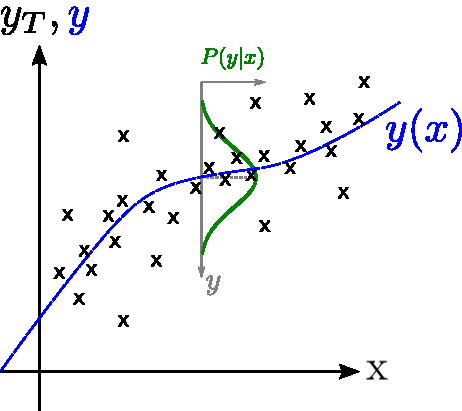
\includegraphics[width=0.4\textwidth]{img/gaussian_labels}
	%\caption{Gaussian distributed labels}
	%\label{fig:gaussian_labels}
%\end{figure}

\begin{figure}[ht]
     \centering
     \savebox{\imagebox}{
	 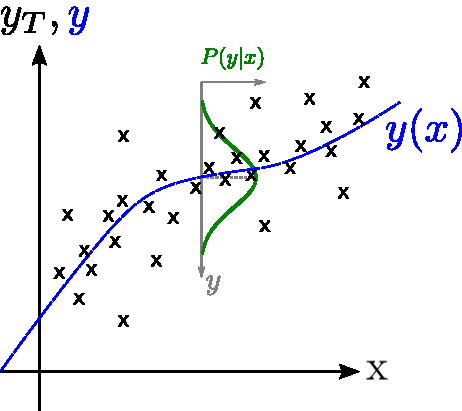
\includegraphics[width=0.37\textwidth]{img/gaussian_labels}}%
     \begin{subfigure}[t]{0.37\textwidth}
         \centering
         \usebox{\imagebox}% Place largest image
         \caption{guassian labels}
         \label{fig:quadratic}
     \end{subfigure}
     \hspace{2mm}
     \begin{subfigure}[t]{0.37\textwidth}
         \centering
         \raisebox{\dimexpr.5\ht\imagebox-.5\height}{% Raise smaller image into place
         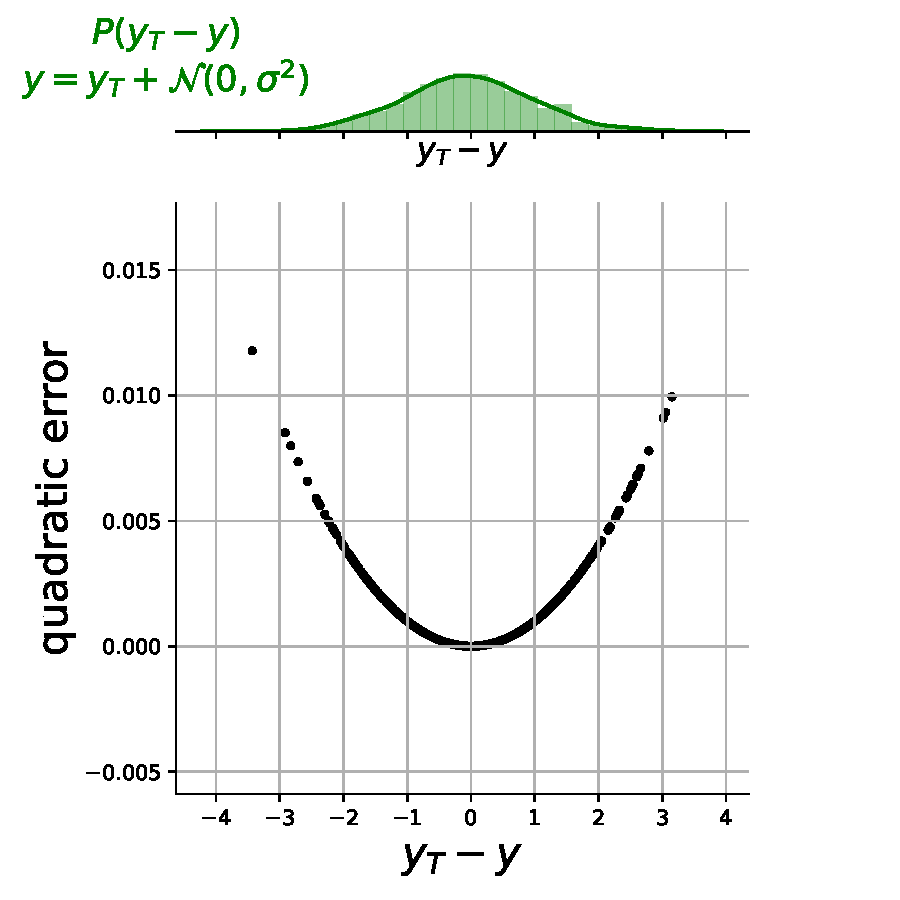
\includegraphics[width=0.99\textwidth]{img/qudaratic_conditional}
         }
         \caption{aggregate density}
         \label{fig:linear}
     \end{subfigure}
     \mode<article>{
     \caption{quadratic error and guassian labels}
     }
	 \label{fig:quadratic_density_gaussian}
\end{figure}
}
\only<4>{
\begin{align}
\vec w^* \in \argmin_{\vec w} \ETw 
\iff& 
\argmax_{\vec w} \underbrace{\prod_{\alpha=1}^{p} \mathcal{N}(y_T|{y(\vec x;\vec w)},\sigma^2)
}_{
\text{likelihood function } \mathcal{L(\vec w)}
}\\
&=
\argmin_{\vec w}
\underbrace{
 \lbrack - \ln \mathcal{L(\vec w)}\rbrack
 }_{\text{neg. log likelihood}}
\end{align} 
}


\end{frame}

\mode<article>{
This property makes the quadratic cost function the standard choice for regression.
}

\subsubsection{Cost functions for binary classification}

\begin{frame}\frametitle{\subsubsecname\\Deriving the cross entropy cost function for binary classification}

\mode<article>{
\textbf{Deriving the cross entropy cost function for binary classification}
}

\begin{itemize}
\item[]\underline{Data}:\\

\begin{equation}
\Big\{ \left( \vec x^{(\alpha)}, y_T^{(\alpha)} \right) \Big \}_{\alpha=1}^{p}
\end{equation}

with 
$$
\vec x^{(\alpha)} \in \R^N\;\;,\;\; y_T^{(\alpha)} \in \{{\color{red}0}, {\color{blue}1}\}.
$$

generated by
\begin{equation}
\left( \vec x^{(\alpha)}, y_T^{(\alpha)} \right) \stackrel{\iid}{\sim} P_{\text{data}}(\vec x, y)
\end{equation}

\pause

\item[]\underline{Model}:\\

MLP, scalar output \mode<article>{interpreted as probability that $y(\vec x; \vec w)=1$. In other words the probability of $\vec x$ belonging to class '1' (the positive class):}

\begin{equation}
y(\vec x;\vec w) =: P_{\text{model}} ({\color{blue}y=1}|\vec x;\vec w) \;\; \text{and} \;\; P_{\text{model}} ({\color{red}y=0}|\vec x; \vec w) = 1-y(\vec x;\vec w)
\end{equation}

for the \textcolor{blue}{``positive''} and \textcolor{red}{``negative''/``other''} class respectively.

\end{itemize}

\end{frame}

\begin{frame}\frametitle{Cost function derivation via minimization of \\the Kullback-Leibler divergence}

\mode<article>{
\textbf{The Kullback-Leibler divergence }

}

$\dkl(P||Q)$ is a measure of how much a probability distribution $P$ differs from another distribution $Q$.

\begin{align}
\dkl\left(\, P( z) ||\, Q( z) \,\right)
:= \int d  z \, P( z)
\ln 
\left( 
\frac{P(z)}{Q(z)}
\right)
\end{align}

\only<1>{
\begin{center}
	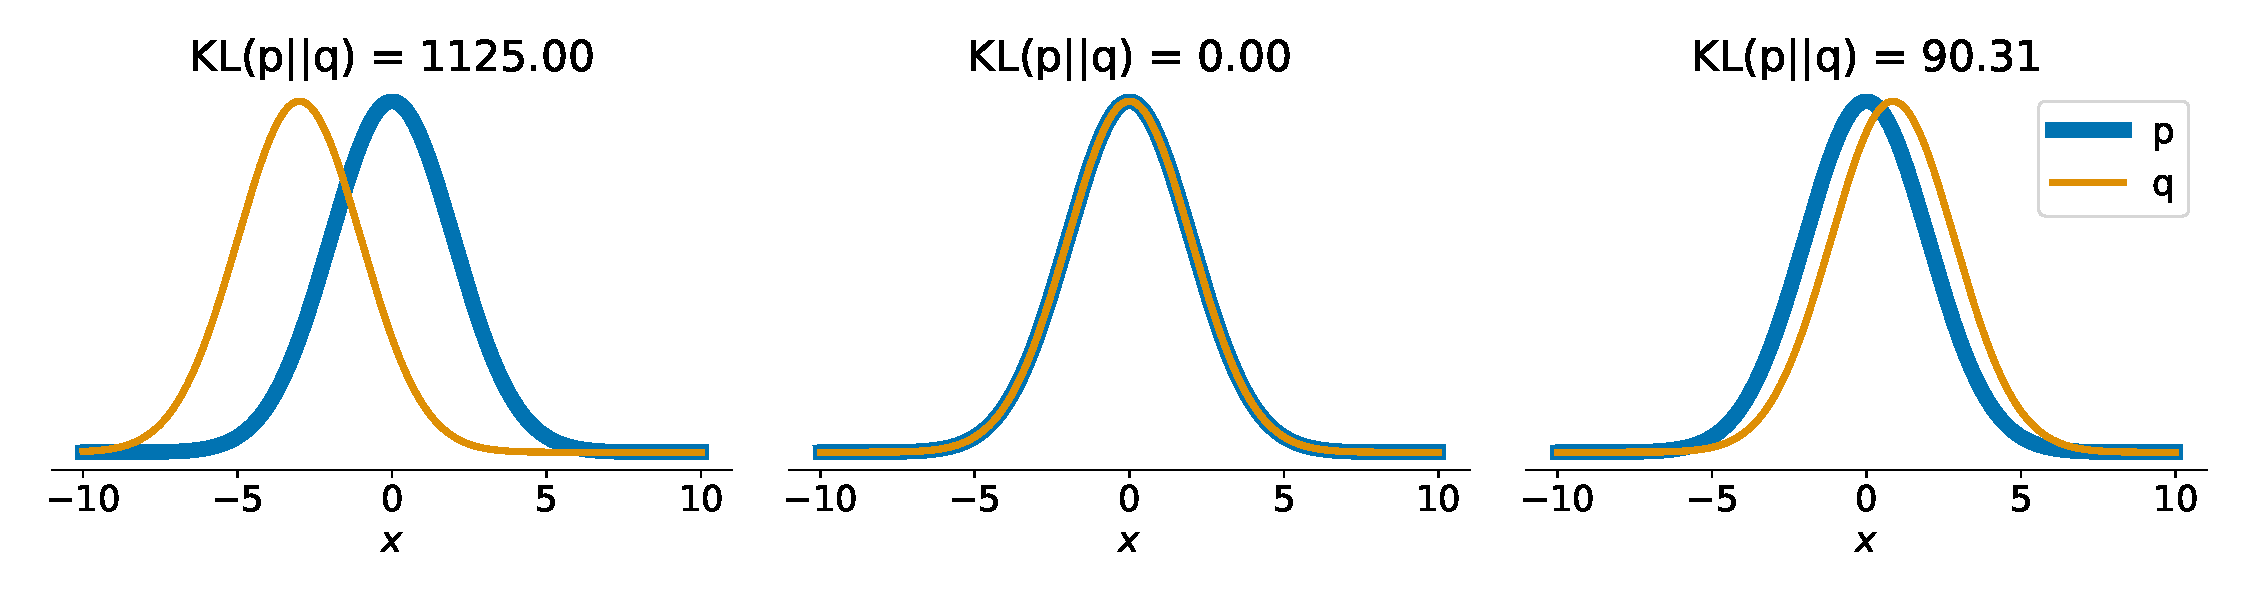
\includegraphics[width=0.7\textwidth]{img/kl_normal}
	\notesonly{\captionof{figure}{The KL divergence for comparing two distributions.}
	}
\end{center}
}
\only<2>{
Properties of the KL-divergence:

\begin{itemize}
\item $\dkl = 0$ iff. both distribution are \emph{identical},
\item otherwise, $\dkl > 0$.
\item[!] Does not qualify as a metric because it is not symmetric. For different distributions $P$ and $Q$:
	\begin{equation}
	\dkl(P||Q) \ne \dkl(Q||P)
	\end{equation}
\end{itemize}
}

\end{frame}

\begin{frame}\frametitle{Cost function derivation via minimization of the Kullback-Leibler divergence}
 
From KL-divergence to binary cross entropy loss:
\only<1>{

\begin{align}
\dkl\left(\, P_{\text{data}}(\vec x, y) \,||\, P_{\text{model}}(\vec x, y) \,\right)
= \iint d \vec x dy P_{\text{data}}(\vec x, y)
\ln 
\left( 
\frac{P_{\text{data}}(\vec x, y)}{P_{\text{model}}(\vec x, y)}
\right)
\end{align}

\mode<article>{
Integrating w.r.t. $y$ $\corresponds$ sum over the set of all possible values for $y$, which is $\{0,1\}$ in this case:
}
}
\definecolor{darkgreen}{rgb}{0,0.6,0}
\begin{align}
\only<1,2>{
\dkl&\left(\, P_{\text{data}}(\vec x, y) \,||\, P_{\text{model}}(\vec x, y) \,\right)\\
&= \int_{\R^N} d \vec x \sum_{y \in \{0,1\}} P_{\text{data}}(\vec x, y) \ln 
\left( 
\frac{P_{\text{data}}(\vec x, y)}{P_{\text{model}}(\vec x, y)}
\right)\\
}
\only<1,2>{
&= \int_{\R^N} d \vec x \sum_{y \in \{0,1\}} 
	\underbrace{
		P_{\text{data}}(\vec x)P_{\text{data}}(y | \vec x)
	}_{
		\substack{
		=P_{\text{data}}(\vec x, y)\\(\text{Bayes' rule})
		}
	}
	\ln 
	\left( 
		\frac{ P_{\text{data}}(\vec x)P_{\text{data}}(y | \vec x) }
		{
		\smash{
			\underbrace{
				P_{\hcancel[red]{\text{model}}}(\vec x)
				}_{
				\substack{
					\color{red}\text{discriminative model}\\
					\color{red}\text{not a generative model}\\
					\color{red}\text{replace with }
					{\color{cyan} P_{\text{data}}(\vec x)}
				}%substack
			}%underbrace
			\hspace{-5mm}
			P_{\text{model}}(y | \vec x)
		}%smash
		}%frac(lower)
	\right) \\
}
\only<2,3,4>{
&= \int_{\R^N} d \vec x \sum_{y \in \{0,1\}} 
	\underbrace{
		\color{darkgreen}
		P_{\text{data}}(\vec x)
	}_{\text{indep. of } y}
	P_{\text{data}}(y | \vec x)
	\ln 
	\left( 
	\frac{
		{ \color{cyan} P_{\text{data}}(\vec x) }
		{ \color{violet} P_{\text{data}}(y | \vec x) }
	}
	{
		{ \color{cyan} P_{\text{data}}(\vec x) }
		{ \color{brown} P_{\text{model}}(y | \vec x) }
	}%frac(lower)
	\right) \\
}
\only<3,4>{
&= \underbrace{
	\int_{\R^N} d \vec x \,
	{ \color{darkgreen} P_{\text{data}}(\vec x) }
	\sum_{y \in \{0,1\}}
	P_{\text{data}}(y | \vec x)
	\ln 
	\lbrack { \color{violet} P_{\text{data}}(y | \vec x) } \rbrack
	}_{\text{indep. of model parameters } \vec w} \\
	&\qquad- \int_{\R^N} d \vec x \,
		{ \color{darkgreen} P_{\text{data}}(\vec x) }
		\underbrace{
			\sum_{y \in \{0,1\}}
			P_{\text{data}}(y | \vec x)
			\ln
			\lbrack {\color{brown} P_{\text{model}}(y | \vec x) } \rbrack
		}_{
		\substack{
		\text{\textbf{cross entropy} between } \\
		\text{data \& model distributions given }\vec x}
		}
}
\end{align}

\mode<presentation>{
\only<4>{
Apply ERM on the second term with \textbf{cross entropy}.
}
}

\end{frame}

\begin{frame}\frametitle{ERM}

\mode<article>{
ERM for computing cross entropy loss using the training data:
}
\mode<presentation>{
\vspace{-5mm}
}

\begin{align}
\onslide<1->{
\ETw &= \frac{1}{p} \sum_{\alpha=1}^{p} - \bigg( \;
	\sum_{y\in\{{\color{red}0},{\color{blue}1}\}} P_{\text{data}}(y | \vec x^{(\alpha)})
	 \ln \lbrack P_{\text{model}}(y | \vec x^{(\alpha)}) \rbrack
	 \;\bigg)\\
	 &= \frac{1}{p} \sum_{\alpha=1}^{p} - \bigg( \;
	P_{\text{data}}({\color{blue}y=1} | \vec x^{(\alpha)})
	 \ln \lbrack P_{\text{model}}({\color{blue}y=1} | \vec x^{(\alpha)}) \rbrack \\
	 &\qquad\qquad\qquad+
	 P_{\text{data}}({\color{red}y=0} | \vec x^{(\alpha)})
	 \ln \lbrack P_{\text{model}}({\color{red}y=0} | \vec x^{(\alpha)}) \rbrack 
	  \;\bigg)\\
}
\onslide<2->{
	 &= \frac{1}{p} \sum_{\alpha=1}^{p} - \bigg( \;
		{\color{blue}y_T^{(\alpha)}} \cdot
	 \ln \lbrack {\color{blue}y(\vec x^{(\alpha)};\vec w)} \rbrack
	 + ( {\color{red}1-y_T^{(\alpha)}} ) \cdot
	 \ln \lbrack {\color{red}1-y(\vec x^{(\alpha)};\vec w)} \rbrack
	 \;\bigg)\\
}
\onslide<3->{
	 &= \frac{1}{p} \sum_{\alpha=1}^{p} \bigg( -
		{\color{blue}y_T^{(\alpha)}} \cdot
	 \ln \lbrack {\color{blue}y(\vec x^{(\alpha)};\vec w)} \rbrack
	 - ( {\color{red}1-y_T^{(\alpha)}} ) \cdot
	 \ln \lbrack {\color{red}1-y(\vec x^{(\alpha)};\vec w)} \rbrack  \;\bigg) \\
	 \notesonly{
	 &= \frac{1}{p} \sum_{\alpha=1}^{p} e\tyxwalpha
	 }
}
\end{align}

Extendable to multi-class cross entropy alongside \emph{softmax} normalization.

\end{frame}

\newpage

\begin{frame}
    
{
\notesonly{
\renewcommand{\arraystretch}{1.4} %<- control vertical spacing
}
\slidesonly{
\renewcommand{\arraystretch}{1.2} %<- control vertical spacing
}
\begin{center}
%\begin{table}[h!]
\notesonly{\captionof{table}{Cost functions \& output layers}\slidesonly{\vspace{-5mm}}}
\resizebox{0.9\textwidth}{!}{%
\hskip-2.0cm
\begin{tabular}{|l|c|c|l|}
\hline
task 
&  
\begin{tabular}[c]{@{}c@{}}\multicolumn{1}{c}
~\\[-5mm]
data\\
$\big\{ \vec x^{(\alpha)}, y_T^{(\alpha)} \big\}_{\alpha=1}^{p}$\\[2mm]
\end{tabular}
& output layer 
& \begin{tabular}[c]{@{}c@{}}
    cost function\\ 
    $e := e\tyxw$\end{tabular} \\ 
\hline \hline
scalar regression 
& 
$y_{T} \in \R$
& \begin{tabular}[c]{@{}l@{}}linear\\ $y = {\vec w^{LL-1}}^{\top} \vec s^{L-1}$\end{tabular} 
& \begin{tabular}[c]{@{}c@{}}quadratic error\\
$e = \frac{1}{2} \big( y_{T} - y\big)^{2}$\end{tabular} 
\pause
\\ \hline
\begin{tabular}[c]{@{}l@{}}multivariate linear \\ regression\end{tabular} 
&  
$\vec y_{T} \in \R^{M}$
& \begin{tabular}[c]{@{}l@{}}linear\\ $y_{k} = {\vec w_{k}^{LL-1}}^{\top} \vec s^{L-1}$\end{tabular} 
& \begin{tabular}[c]{@{}c@{}}squared Euclidean \\ distance\\ 
$e = \frac{1}{2} \lVert \vec y_{T} - \vec y \rVert^{2}_{2}$
\end{tabular}
\pause
\\ \hline
\begin{tabular}[c]{@{}l@{}}binary \\ classification\end{tabular} 
&  $y_{T} \in \{0,1\}, \{-1,1\}$
&
\begin{tabular}[c]{@{}c@{}}logistic sigmoid\\ 
$y = \frac{1}{1+exp(-h_{1}^{L})}$\\
or $y = \tanh(h_{1}^{L})$
\end{tabular} 
& \begin{tabular}[c]{@{}l@{}}cross entropy\\ 
$
e = \kern-.5ex
- y_T
\ln \lbrack y \rbrack \quad$\\
$
\;
-\kern-.2ex ( 1\kern-.5ex-\kern-.5exy_T )
\ln \lbrack 1\kern-.5ex-\kern-.5exy \rbrack
$
\end{tabular}
\pause
\\ \hline
\begin{tabular}[c]{@{}l@{}}multi-class \\ classification\\ with $M$ classes\end{tabular} 
&  
\begin{tabular}[c]{@{}c@{}}
$\vec {y}_{T} \in \{0,1\}^{M}$\\
1-out-of-$M$ encoding/\\
1-hot-encoding\\
e.g. $\vec {y}_{T}=(0,0,1,0)^{\top}$\\ $\corresponds$ class 3 out of 4
\end{tabular}
& \begin{tabular}[c]{@{}c@{}}softmax\\ 
$y_{k} = \frac{exp(h_{k}^{L})}{\sum_{k=1}^{M} exp(h_{k}^{L})}$\\[5mm]
$\Rightarrow \sum_{k=1}^{M} y_{k} = 1$
\end{tabular}
& \begin{tabular}[c]{@{}c@{}}cross entropy\\(multi-class case)\\ 
$
e = \kern-.3ex
-\kern-.2ex\sum_{k=1}^{M} {y_T}_{k} $\\
$\;\;\cdot 
%$\cdot
\ln \lbrack y_{k}\big(\vec x; \vec w\big) \rbrack
$
\end{tabular} \\
\hline
\end{tabular}
}
%\end{table}
\end{center}
} % arraystretch

\end{frame}
